\chapter{Metallurgie}	

\section{Metallurgie von Titan und Titanlegierungen (PH)}
\label{Titanallg}

Reines Titan ist das vierthäufigste Metall in der Erdkruste (etwa 0,4 -- 0,6 \%) und zeigt eine hohe Reaktivität mit anderen Elementen des Periodensystems. Es tritt in zwei verschiedenen Gittermodifikationen auf. Es gibt die $\alpha$-Phase, die ein hexagonales Gitter annähernd dichtester Kugelpackung (hex) aufweist. Außerdem gibt es die $\beta$-Phase, die eine kubisch-raumzentrierte Gitterstruktur (krz) besitzt (Abbildung \ref{fig:Kristallgitter}). Bei einer Temperatur von $882 \pm 2 ^\circ C$ tritt eine Phasenumwandlung von $\alpha$ zu $\beta$ auf. Die Temperatur, bei der diese Umwandlung stattfindet, ist eine wichtige Kenngröße im Bereich der Titanwerkstoffe und wird $\beta$-Transus-Temperatur ($T_{\beta}$) genannt.
Die Umwandlung $\beta$ zu $\alpha$ kann durch einen diffusionskontrollierten Keimbildungs- und Wachstumsprozess oder durch einen diffusionslosen Umklappvorgang (martensitisch) erfolgen, wenn eine ausreichend schnelle Abkühlgeschwindigkeit (über 500 K/s) erzielt wird \cite{C.Leyens.2005,Lutjering.2007}.

\begin{figure}[h]
	\centering
	\subfloat{}
	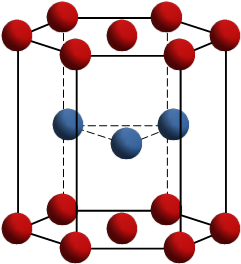
\includegraphics[width=0.3\textwidth]{./Bilder/hcp}
	\hspace{4ex}
	\subfloat{}
	\includegraphics[width=0.3\textwidth]{Bilder/krz}
	\caption{Kristallgitterstruktur der $\alpha$-Phase (hex) und $\beta$-Phase (krz)}
	\label{fig:Kristallgitter}
\end{figure}

\subsection{Klassifizierung von Titan und Titanlegierungen}

Da reines Titan wie alle anderen Metalle keine hohe Festigkeit besitzt, werden Legierungen hergestellt, um die mechanischen Eigenschaften gezielt zu verändern. Die in der Industrie erhältlichen Titanlegierungen werden daher in verschiedene Klassen eingeteilt. Es gibt technisch reines Titan (CP-Titanium), $\alpha$-, $\alpha+\beta$-, metastabile $\beta$- sowie die $\beta$-Legierungen. Des Weiteren gibt es die near-$\alpha$- und near-$\beta$-Legierungen. Für die Klassifikation ist der Anteil an $\beta$-Phase im Gefüge bei Raumtemperatur entscheidend.
Die für Titanwerkstoffe typischen Legierungselemente werden in vier Kategorien eingeteilt, die sich in ihrer Wirkungsweise unterscheiden. 
Als $\alpha$-Stabilisatoren werden Legierungselemente wie Aluminium (Al), Sauerstoff (O) und Stickstoff (N) bezeichnet, die zu einer Einschnürung des $\beta$-Phasengebietes führen und die $\beta$-Transus-Temperatur erhöhen.
Des Weiteren gibt es die $\beta$-Stabilisatoren, die das $\beta$-Phasengebiet erweitern und die $\beta$-Transus-Temperatur verringern. Man unterscheidet bei den $\beta$-Stabilisatoren zwischen $\beta$-isomorphen und $\beta$-eutektoiden Stabilisatoren. Zu den $\beta$-isomorph wirkenden Stabilisatoren gehören die Elemente Molybdän (Mo), Vanadium (V), Niob (Nb) und Tantal (Ta). Diese erweitern das $\beta$-Phasengebiet bis zur Raumtemperatur. 
Zu den $\beta$-eutektoiden-Stabilisatoren gehören Elemente wie Eisen (Fe), Chrom (Cr), Kupfer (Cu), Mangan (Mn) und Silizium (Si). Bei diesen Stabilisatoren kommt es unterhalb einer elementabhängigen Grenztemperatur zu einer eutektoiden Reaktion, die zu einer Ausscheidung einer zusätzlichen Phase führt. Die Elemente Zinn (Sn) und Zirkon (Zr) werden häufig als neutral bezeichnet, da diese nur eine sehr geringe $\alpha$-stabilisierende Wirkung haben. Einen Überblick über den Einfluss der Legierungselemente auf $\alpha$- und $\beta$-Phase gibt die Abbildung \ref{fig:tabelle-1}.

\begin{figure}[h]
	\centering
	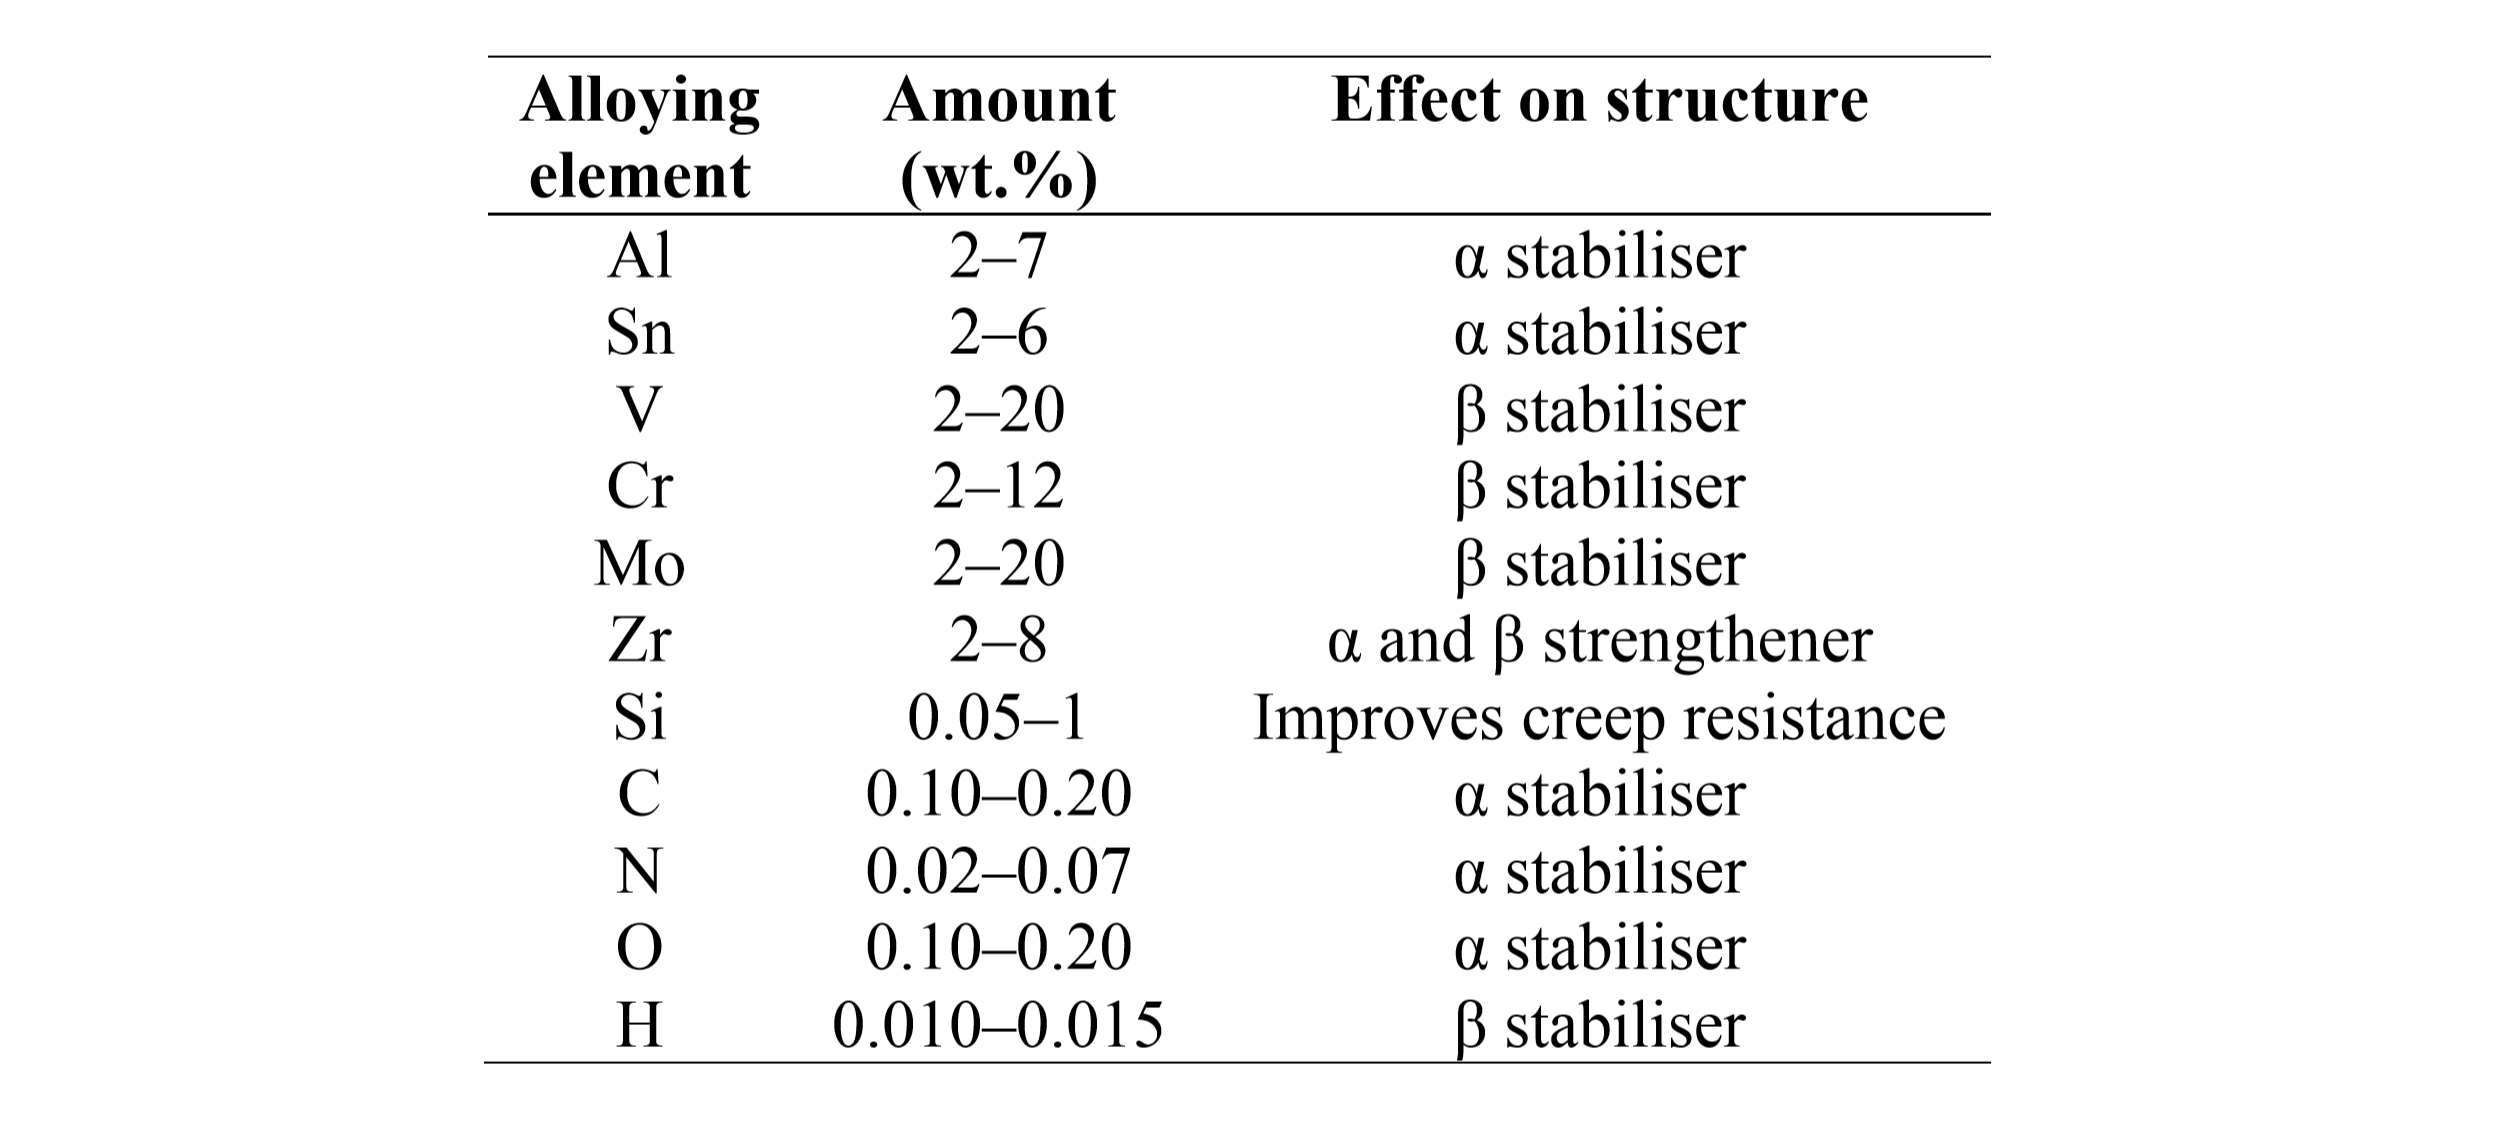
\includegraphics[width=0.9\linewidth]{./Bilder/Tabelle 1.png}
	\caption{Einfluss der Legierungselemente auf $\alpha$- und $\beta$-Phase (schematisch) \cite{Lutjering.2007}}
	\label{fig:tabelle-1}
\end{figure}

Bei einer Wärmebehandlung von near-$\alpha$-, $\alpha$+$\beta$- oder metastabilen $\beta$-Titanlegierungen im Zweiphasengebiet (also unterhalb der $\beta$-Transus-Temperatur) kommt es bei ausreichend langen Glühzeiten zum sogenannten Element Partitioning \cite{Lutjering.2007}. Dabei diffundieren die $\alpha$-stabilisierenden Elemente in die $\alpha$-Phase und die $\beta$-stabilisierenden Elemente in die $\beta$-Phase, sodass die lokale chemische Zusammensetzung der jeweiligen Phasen von der globalen chemischen Zusammensetzung einer Legierung abweichen kann.



\paragraph{CP-Titanium} 
Technisch reines Titan (\textit{commercially pure}, CP) enthält nur Sauerstoff und Eisen als zusätzliche Legierungselemente, jedoch sind Begleitelemente/Verunreinigungen in bestimmten Mengen zugelassen und auch nicht zu vermeiden. In welche Klasse technisch reines Titan eingeordnet wird, hängt von der chemischen Zusammensetzung ab. Es gibt 4 Klassen, die sogenannten CP-Grades \cite{C.Leyens.2005}.

\paragraph{$\alpha$- und near-$\alpha$-Legierungen}
Werden $\alpha$-Stabilisatoren dem reinen Titan hinzulegiert, führt dies zu den sogenannten $\alpha$-Legierungen. Wird ein kleiner Anteil an $\beta$-Stabilisatoren ( 1--2 Gew.\%) hinzugefügt, führt dies zu einer near-$\alpha$-Legierung mit einem kleinen Anteil an $\beta$-Phase (\textless5\%) bei Raumtemperatur. Ein typisches Beispiel einer $\alpha$-Legierung ist Ti–5Al–2.5Sn. Zu den Vertretern von near-$\alpha$-Legierungen gehören Ti–8Al–1Mo–1V und Ti–6Al–2Sn–4Zr–2Mo. Der Aluminiumgehalt in diesen Legierungen wird typischerweise unter 9\% gehalten, da es sonst zu Ti$_3$Al-Ausscheidungen und dadurch zu Versprödungen kommen kann \cite{C.Leyens.2005,Lutjering.2007,Boyer.2007,M.J.Donachie.2010}.

\paragraph{$\alpha$+$\beta$-Legierungen}
Diese Legierungen bilden die erste Untergruppe der zweiphasigen Titanlegierungen. Bei Raumtemperatur besitzen sie zwischen 5\% und 35\% $\beta$-Phase im Gefüge. Sie können dabei vollständig oder teilweise martensitsch ($\alpha'$- oder $\alpha''$-Phase) umwandeln. Die bekanntesten $\alpha$+$\beta$-Legierungen sind Ti–6Al–4V und Ti–6Al–2Sn–4Zr–6Mo \cite{C.Leyens.2005,Lutjering.2007,Boyer.2007,M.J.Donachie.2010}.

Die metastabilen $\beta$-, near-$\beta$- und $\beta$-Legierungen werden an dieser Stelle nicht näher erläutert, da sie für diese Arbeit nicht relevant sind.

\subsection{Mikrostrukturen in Titanlegierungen}
Im Bereich der Titanlegierungen gibt es drei Basis-Mikrostrukturen, die eingestellt werden können. Es gibt lamellare, globulare und Bi-modal/Duplex-Gefüge \cite{C.Leyens.2005,Lutjering.2007,Boyer.2007,M.J.Donachie.2010}.

Mikrostrukturen, die man während des Gießens erhält, sind sehr grob und besitzen eine geringe Festigkeit. Daher werden diese Mikrostrukturen mithilfe von thermo-mechanischen Prozessschritten gezielt modifiziert. Dazu gehören die Verfeinerung der Mikrostruktur durch Rekristallisation oder die Formation neuer Mikrostrukturen durch Kornwachstum \cite{C.Leyens.2005,Lutjering.2007,Boyer.2007,M.J.Donachie.2010}.

Typische thermo-mechanische Prozessschritte für near-$\alpha$- und $\alpha+\beta$-Legierungen beinhalten die Homogenisierung (solution heat treatment), Deformation, Rekristallisation, das Altern (ageing) und Spannungsarmglühen (stress relief annealing). Die $\beta$-Transus-Temperatur spielt dabei eine entscheidende Rolle, welche Gefüge sich bei den Legierungen einstellen \cite{C.Leyens.2005,Lutjering.2007,Boyer.2007}.
 
Eine kurze Beschreibung dieser Mikrostrukturen ist im folgenden aufgeführt.

\begin{itemize} 
	\item lamellare Mikrostruktur: Das Glühen und Abschrecken oberhalb der $\beta$-Transus-Temperatur (Abbildung \ref{fig:gefuge-phasendiagramm}) führt zu einer vollständigen martensitischen Umwandlung. Das entstandene Gefüge liegt dann metastabil in der $\alpha'$-Phase vor. Ein Beispiel für diese lamellare Mikrostruktur zeigt Abbildung \ref{fig:abbildung-3}. Bei einer langsamen Abkühlung von oberhalb der $\beta$-Transus-Temperatur stellt sich ein sogenanntes Widmannstättengefüge ein. So bilden sich beim Unterschreiten der $\beta$-Transus-Temperatur an bevorzugten Stellen $\alpha$-Keime, die in die $\beta$-Körner hineinwachsen. Aufgrund von Orientierungsbeziehungen zwischen $\alpha$- und $\beta$-Phase wachsen die $\alpha$-Körner in eine Vorzugsrichtung. Dadurch ensteht ein lamellares Gefüge, dass aus $\alpha$-Lamellen besteht und von schmalen Bereichen von $\beta$-Phase umschlossen ist.
	
\item globulare Mikrostruktur: Bei einer abschließenden Wärmebehandlung im Zweiphasengebiet mit tiefen Temperaturen (Abbildung \ref{fig:gefuge-phasendiagramm}) ist der Anteil an Primär-$\alpha$ im Gefüge höher. Diese globularen $\alpha$-Körner werden dann nur von einem schmalen Rand von $\beta$-Phase umschlossen \cite{Lutjering.2007}. Abbildung \ref{fig:abbildung-5} zeigt ein Beispiel eines globularen Gefüges.

\item bi-modale Mikrostruktur: Das bi-modale oder Duplex-Gefüge entsteht, wenn knapp unterhalb der $\beta$-Transus-Temperatur (Abbildung \ref{fig:gefuge-phasendiagramm}) geglüht und anschließend an der Luft abgekühlt wird. Beim Glühen in diesem Temperaturbereich besteht das Gefüge aus globularen $\alpha$- und $\beta$-Körnern. Beim Abkühlen wandeln die $\alpha$-Körner nicht mehr um, da sie sich bereits in der $\alpha$-Phase befinden, die bei tiefen Temperaturen beständig ist. Diese werden daher als Primär-$\alpha$ oder $\alpha_p$ bezeichnet. Aus der $\beta$-Phase scheidet sich beim Abkühlen $\alpha$-Phase in Form von Lamellen aus. Man spricht dann von transformiertem $\beta$. Bereiche, in denen Lamellen dicht beieinander liegen mit gleicher Orientierungsrichtung nennt man $\alpha$-Lamellenpakete \cite{Lutjering.2007}. Abbildung \ref{fig:abbildung-4} zeigt ein bi-modales Gefüge von Ti-6242. 

\begin{figure}[h]
	\centering
	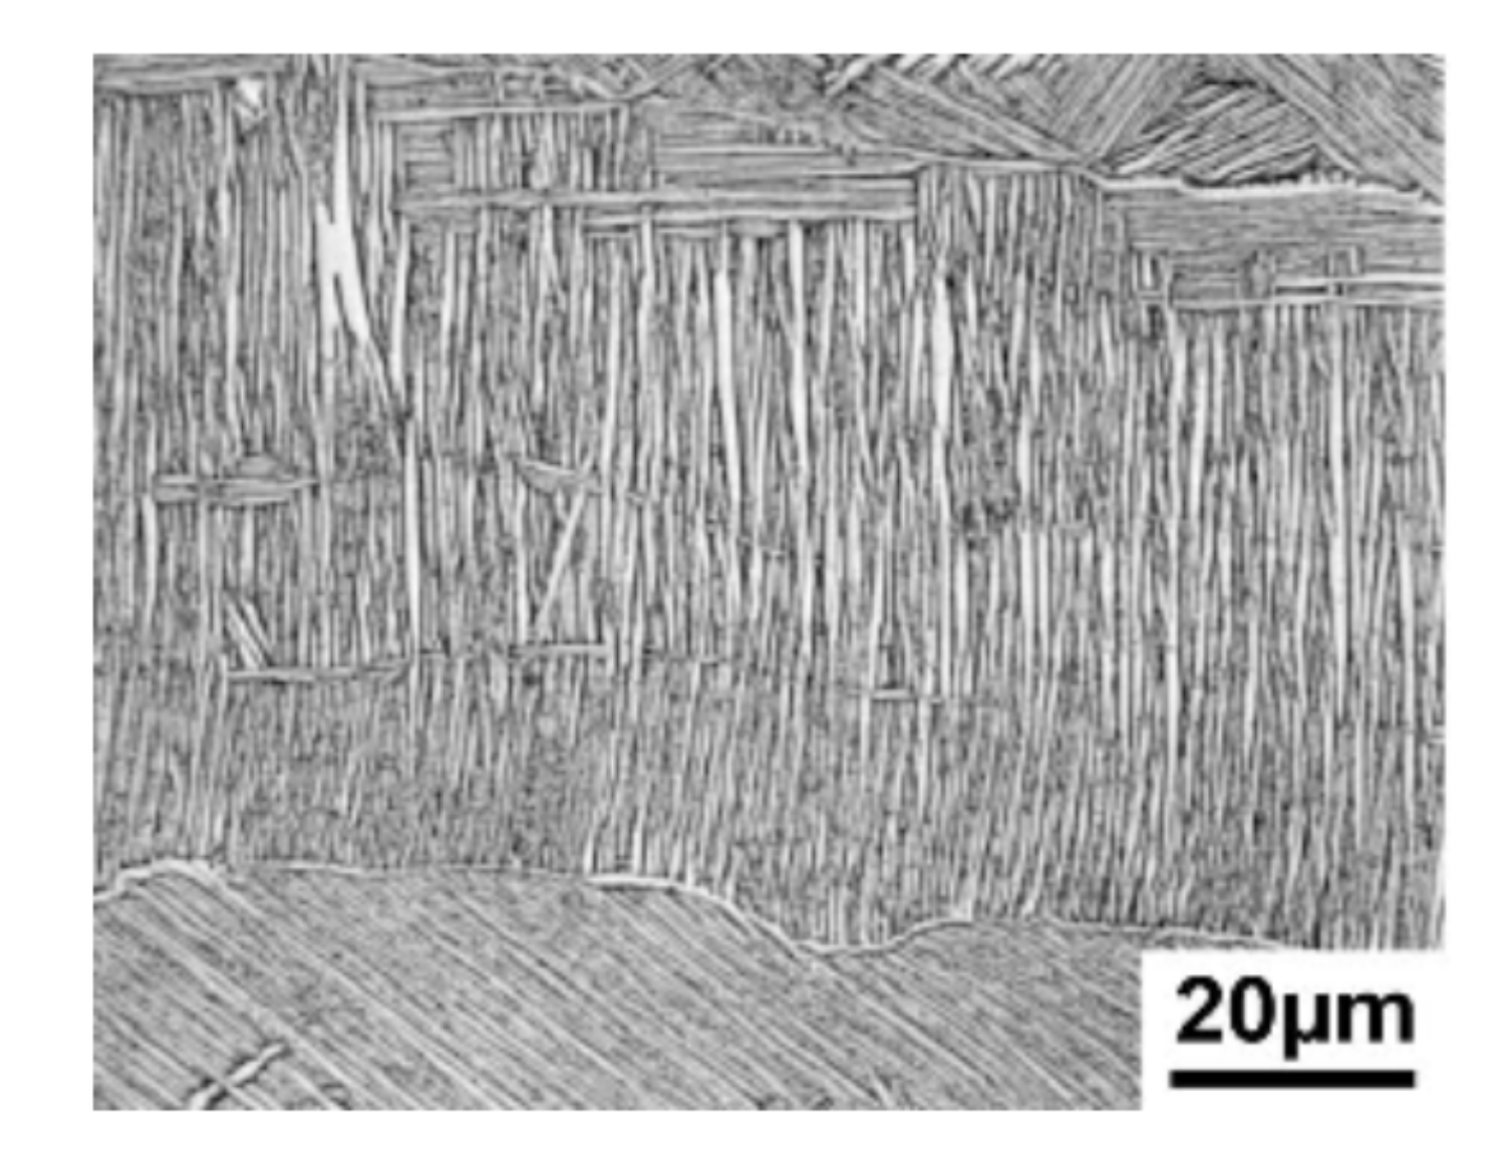
\includegraphics[width=0.6\linewidth]{./Bilder/Abbildung 3.png}
	\caption[Abbildung 3]{lamellare Mikrostruktur von Ti-6242, Abkühlrate ca 100$^\circ$C/min \cite{Lutjering.2007}}
	\label{fig:abbildung-3}
\end{figure}

\begin{figure}[h]
	\centering
	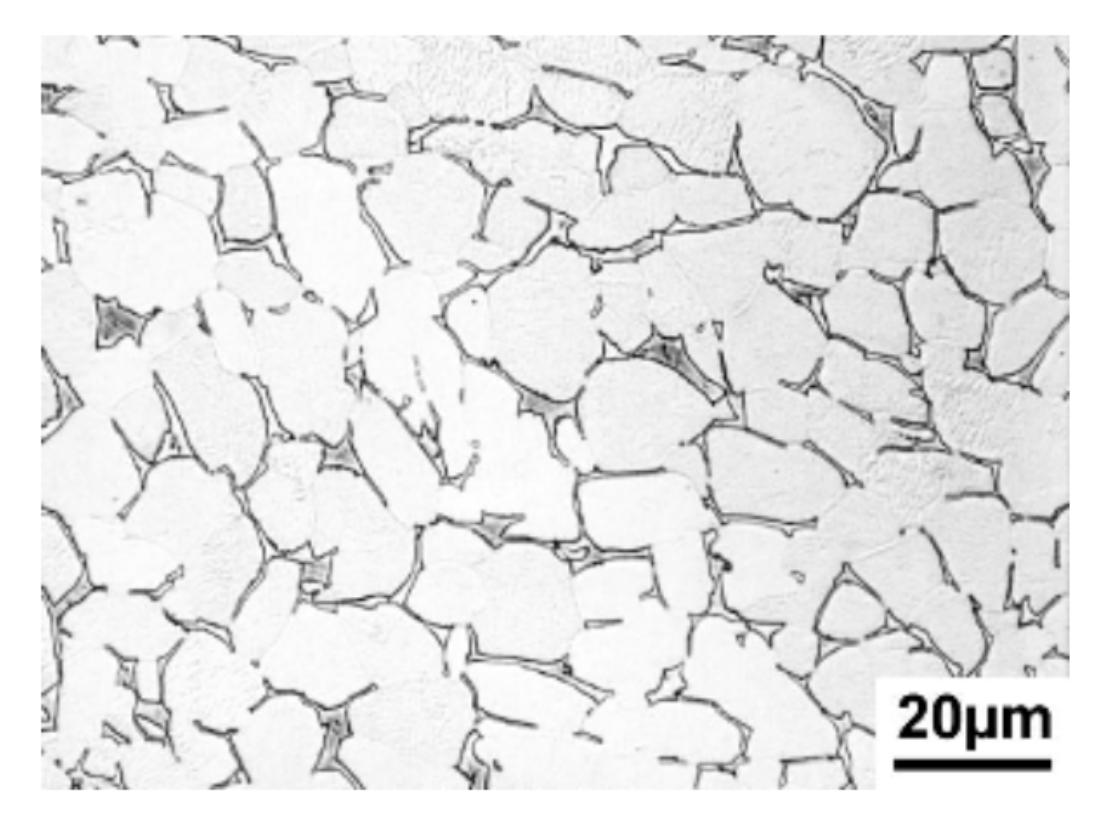
\includegraphics[width=0.6\linewidth]{./Bilder/Abbildung 5.png}
	\caption[Abbildung 5]{globulare Mikrostruktur von Ti-6242 \cite{Lutjering.2007}}
	\label{fig:abbildung-5}
\end{figure}

\pagebreak

\begin{figure}[h]
	\centering
	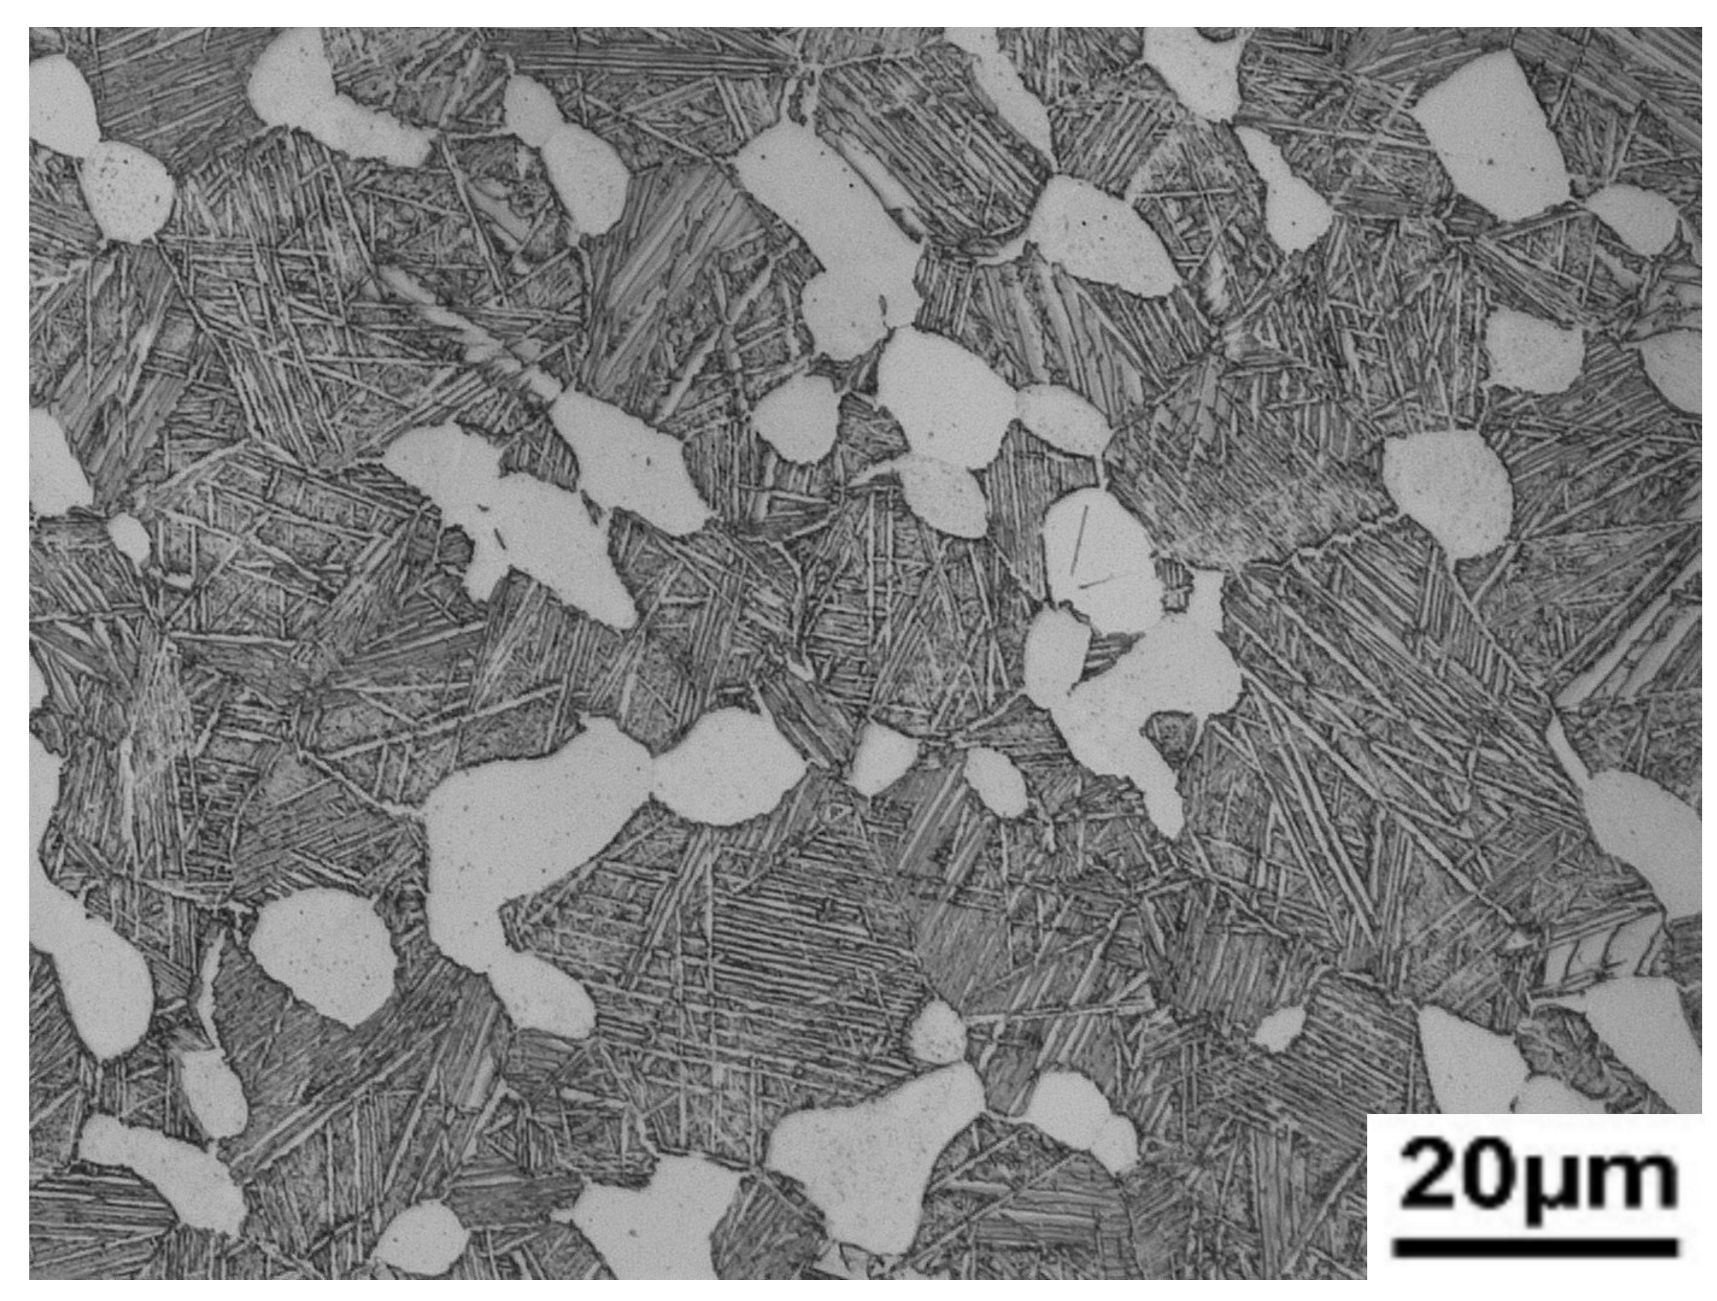
\includegraphics[width=0.5\linewidth]{./Bilder/Abbildung 4.png}
	\caption[Abbildung 4]{bi-modale von Mikrostruktur Ti-6242}
	\label{fig:abbildung-4}
\end{figure}

\end{itemize} 

\begin{figure}[h]
	\centering
	\includegraphics[width=0.9\linewidth]{./Bilder/Gefüge-Phasendiagramm.png}
	\caption{Quasi-binäres Phasendiagramm Titan mit steigendem Anteil an $\beta$-stabilisierenden
    Legierungselementen und die typischen Mikrostrukturen von $\alpha+\beta$-Legierungen}
	\label{fig:gefuge-phasendiagramm}
\end{figure}

\subsection{Eigenschaften von Titanlegierungen}

Dieser Abschnitt gibt einen Überblick über die typischen  Eigenschaften der verschiedenen Klassen von Titanlegierungen.

\paragraph{$\alpha$-Legierungen}  
besitzen eine annehmbare Zugfestigkeit und gute Duktilität bei Raumtemperatur. Des Weiteren besitzen sie eine geringe Dichte, eine gute Härte, sehr gute Kriechbeständigkeit und Schweißbarkeit. Die Besonderheit dieser Legierungen ist, dass sie bei kryogenen Temperaturen keine Versprödung zeigen. CP-Titanium ist die am weitesten genutzte unter den $\alpha$-Legierungen \cite{C.Leyens.2005,Lutjering.2007,M.J.Donachie.2010}.

\paragraph{Near-$\alpha$-Legierungen} 
zeichnen sich durch eine hohe Kriech- und Oxidationsbeständigkeit aus. Ti-6242 ist die am häufigsten kommerziell eingesetzte Legierung für Temperaturen bis zu $550 ^\circ C$. 
Sie wurde als Ergänzung zu der bekannten Ti-64 Legierung entwickelt und erhöhte dadurch das Temperaturlimit. In den meisten near-$\alpha$-Legierungen befindet sich Silizium als Legierungselement, um die Temperaturbeständigkeit zu verbessern \cite{C.Leyens.2005,Lutjering.2007}. 

\paragraph{$\alpha+\beta$-Legierungen} besitzen eine höhere Festigkeit und Härte. Dagegen ist die Duktilität und die Kriechbeständigkeit schlechter als bei near-$\alpha$-Legierungen. Diese Legierungen haben eine hohe Festigkeit bei Raumtemperatur sowie gute Warmumformeigenschaften. Typischerweise besitzen diese Legierungen 10 -- 15 \% $\beta$-Phase bei Raumtemperatur. Ti-64 ist die meistverwendete $\alpha+\beta$-Legierung und besitzt eine gute Kombination aus Festigkeit und Ermüdungseigenschaften bis zu $350 ^\circ C$ \cite{Boyer.2007,M.J.Donachie.2010}. 

Die beschriebenen Eigenschaften der verschiedenen Legierungen sind jedoch abhängig von den zugefügten Legierungselementen sowie dem gewählten Herstellungsprozess.
Die Legierungselemente entscheiden größtenteils über die mechanischen und chemischen Eigenschaften wie Korrosion und Oxidation \cite{C.Leyens.2005,Lutjering.2007,M.J.Donachie.2010}.

Der Herstellungsprozess hat ebenfalls einen erheblichen Einfluss auf die mechanischen Eigenschaften der Legierungen. Durch verschiedene Wärmebehandlungen können dadurch unterschiedliche Mikrostrukturen eingestellt und ihre mikrostrukturellen Eigenschaften verändert werden \cite{C.Leyens.2005,Lutjering.2007,Boyer.2007,M.J.Donachie.2010}.

Wie im vorherigen Kapitel erwähnt, wird zwischen drei Basis-Mikrostrukturen unterschieden. Neben $\alpha$- und $\beta$-Phase kann Titan in weiteren Phasen auftreten, wie dem thermisch induzierten Martensit, der als $\alpha'$-Phase bezeichnet wird. Die wichtigsten Eigenschaften der Mikrostrukturen werden durch die Größe der $\alpha$-Lamellenpakete und die Breite der $\alpha$-Lamellen beeinflusst \cite{C.Leyens.2005,Lutjering.2007,Boyer.2007}. Die Größe der $\alpha$-Lamellenpakete, die durch verschiedene Abkühlraten beeinflusst wird, ist der wichtigste mikrostrukturelle Faktor. Es hat sich gezeigt, dass eine Verringerung der Lamellenpaketgröße, zu einer Verringerung der effektiven Gleitlänge führt. Dadurch wird die Dehngrenze erhöht und die Rissanfälligkeit verringert. Größere $\alpha$-Lamellenpakete erhöhen dagegen den Widerstand gegen Ermüdungsrissausbreitung und die Bruchzähigkeit. Die Größe der $\alpha$-Lamellenpakete wird durch die Größe des ursprünglichen $\beta$-Korns limitiert \cite{C.Leyens.2005,Lutjering.2007,M.J.Donachie.2010}.

\subsection{Verwendung von Titan und Titanlegierungen}
Titanlegierungen werden hauptsächlich in der Luft- und Raumfahrt verwendet, da sie eine gute Kombination aus einem niedrigen Gewicht, hoher Festigkeit, Korrosionsbeständigkeit und einer hohen Temperaturstabilität bieten \cite{C.Leyens.2005,R.R.Boyer.1996,M.PetersJ.KumpfertC.WardC.Leyens.2003}. Die Haupteinsatzgebiete in der Luftfahrt für Titanlegierungen sind Strukturteile der Luftfahrzeugzelle, Fahrwerksteile sowie Komponenten von Flugtriebwerken. Etwa 7 -- 36 \% des strukturellen Gewichts des Rumpfes und der Triebwerke bestehen aus Titanlegierungen \cite{Lutjering.2007}. In Triebwerken werden sie für Triebwerksschaufeln eingesetzt. Für die meisten Komponenten wird die Standardlegierung Ti-6Al-4V verwendet. Für Komponenten, die eine höhere Temperaturbeständigkeit erfordern, werden Legierungen wie Ti–6Al–2Sn–4Zr–2Mo und IMI 834 eingesetzt. Die hohen Material- und Herstellungskosten verhindern einen breiten Einsatz von Titanwerkstoffen in der Automobilindustrie. Sie werden aber vereinzelt für Motorkomponenten oder Fahrwerksteile, wie beispielsweise Federn benutzt. CP-Titanium findet Anwendung in Bereichen, wo die Anforderungen an mechanische Eigenschaften gering sind, aber eine hohe Korrosionsbeständigkeit gefordert ist. Beispiele dafür sind Wärmetauscher, Rohrleitungen oder Meerwasserentsalzungsanlagen \cite{A.D.Khawajia.2008}. Des Weiteren finden CP-Titanium und Titanlegierungen aufgrund der Biokompatibilität von Titan sowie einer guten Dauerfestigkeit und Korrosionsbeständigkeit Anwendung in der Medizintechnik. Sie werden zur Herstellung von Implantaten sowie medizinischen Geräten benutzt \cite{M.GeethaA.K.SinghR.AsokamaniA.K.Gogia.2009}. Ein weiteres Einsatzgebiet sind moderne Schutzwesten, die neben den Aramidfasern auch Titangewebe enthalten, um das Eindringen von Hieb- und Stichwaffen zu verhindern \cite{C.Leyens.2005}.  

\section{Ti-6242 (ZB)}

\subsection{Zusammensetzung}

Ti-6242 ist eine Titanlegierung, die im Jahr 1967 von TIMET eingeführt wurde \cite{ImmanuelFreiherrvonThungen.}. 
Wie im Phasendiagramm in Abbildung \ref{tab:PD-Ti6242} zu erkennen ist, hat die Legierung Ti-6242 bei Raumtemperatur einen hohen $\alpha$-Anteil und wird deshalb als near-$\alpha$-Legierung bezeichnet.
Die genauen Anteile der Legierungselemente kann der Tabelle \ref{tab:Zusammensetzung} entnommen werden. 


\begin{figure}[H]
	\centering
	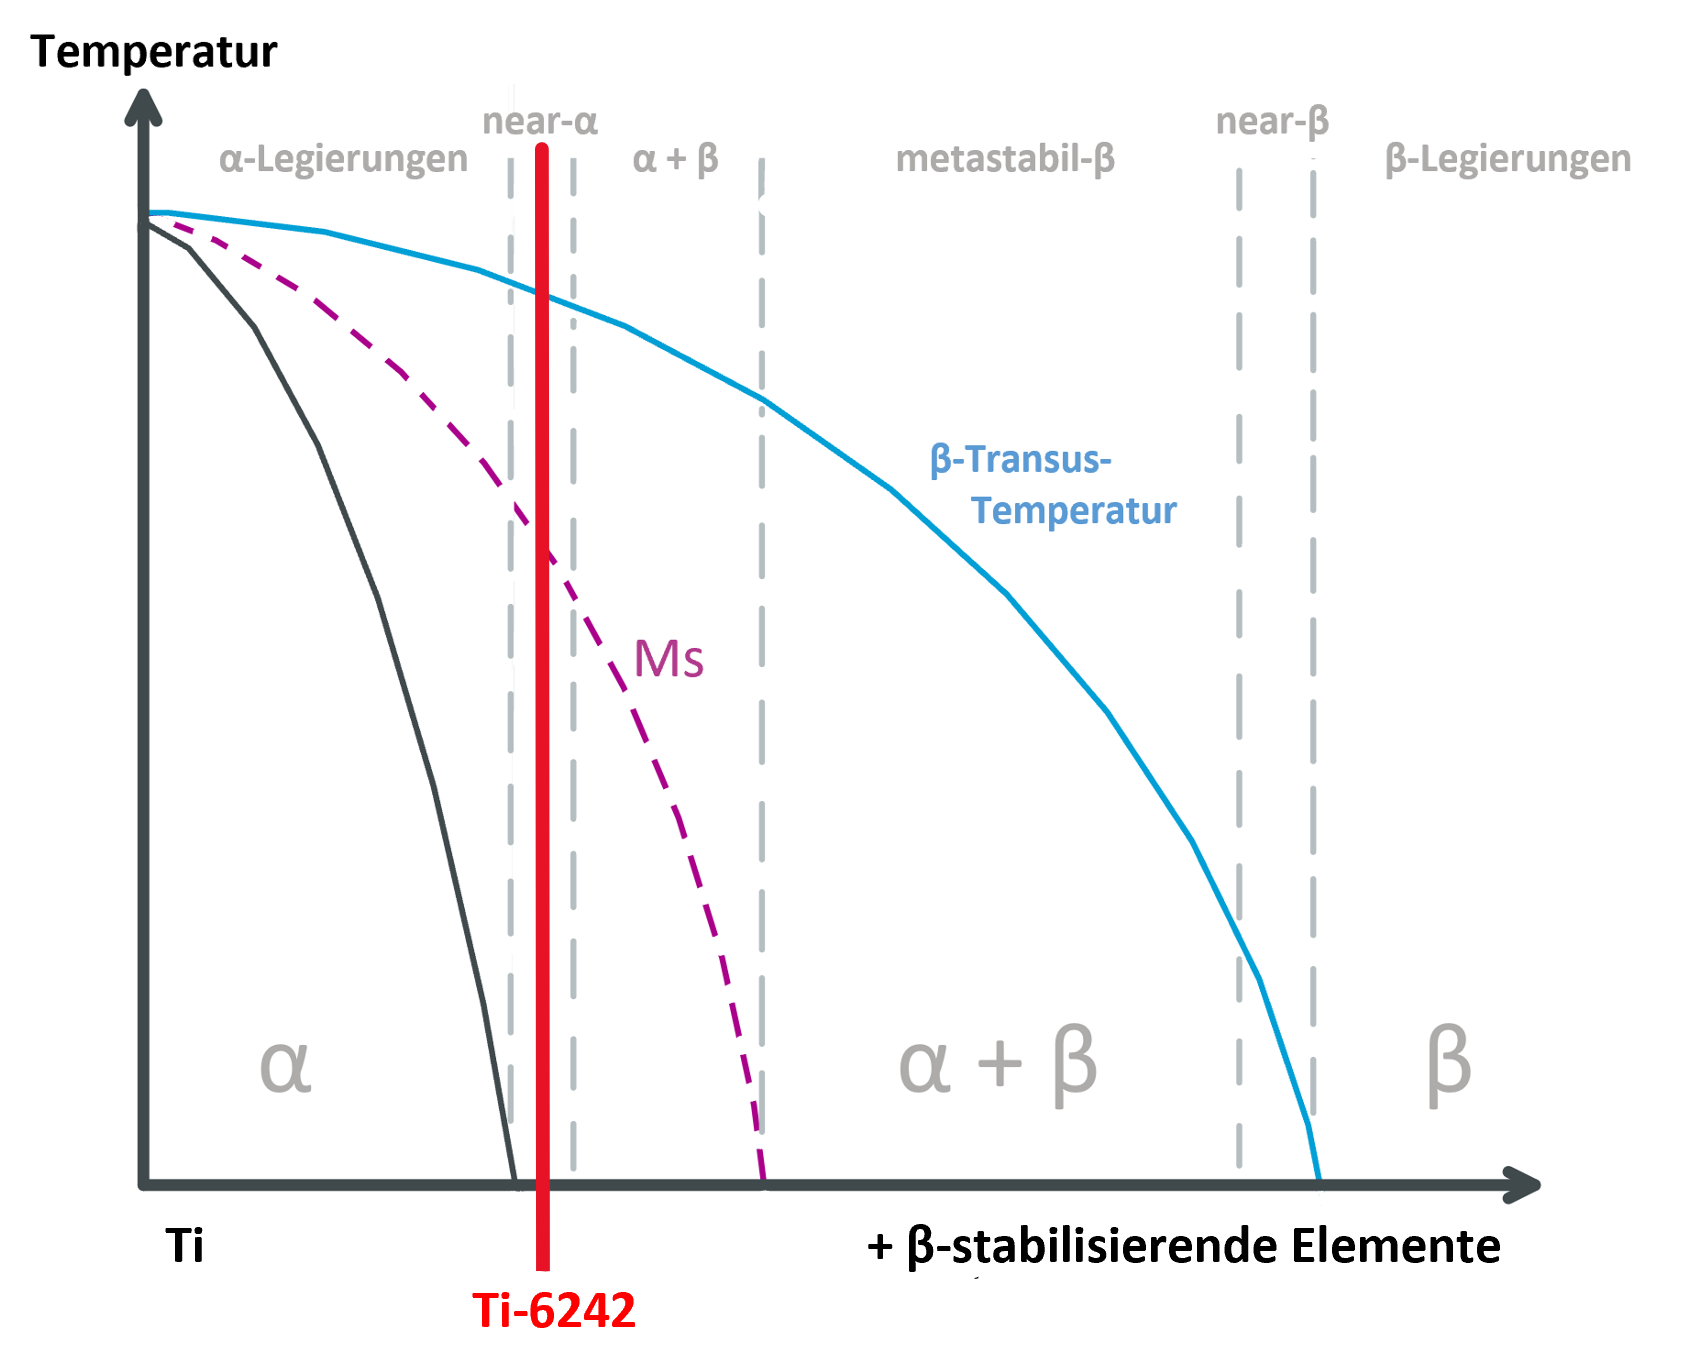
\includegraphics[width=0.7\textwidth]{Bilder/Phasendiagram}
	\caption{Binäres Phasendiagramm Titan und $\beta$-stabilisierende Elemente \cite{M.J.Donachie.2010}}
	\label{tab:PD-Ti6242}
\end{figure}





\begin{table}[h]
	
	\centering	
	\begin{tabular}{|l |c |c|}
		\hline
		\hspace{20ex}Elemente \hspace{20ex} & Min \%Gwt. & Max \%Gwt.\\
		\hline
		Aluminium&5.5&6.5\\
		Zinn&1.80&2.20\\
		Zirkon&3.60&4.40\\
		Molybdän&1.80&2.20\\
		Silizium &0.06&0.13\\
		Eisen&-&0.25\\
		Sauerstoff&-&0.15\\
		Kohlenstoff&	-&	0.05\\
		Stickstoff&-&0.03\\
		Wasserstoff&-&0.0125\\
		
		
		\hline
	\end{tabular}
	\caption{Legierungselemente von Ti-6242 \cite{M.J.Donachie.2010}}
	\label{tab:Zusammensetzung}
\end{table}


Die Ti-6242S ist eine Optimierung von Ti-6242, die in den 1970er Jahren  entwickelt wurde. Zusätzliches Silizium wird in kleinen Mengen zulegiert, um die Resistenz gegen Kriechen vor allem bei hohen Temperaturen durch die Bildung von Siliziden (Ti$_5$Si$_3$) zu erhöhen \cite{C.Leyens.2005}.

%Verzeichnis : [Immanuel Freiherr von Thungen] - Immanuel Freiherr von Thungen. Effet dwell: relation microstructure-microtexture-propriétés mécaniquesdel’alliagedetitaneTi6242. Autre. ISAE-ENSMAEcoleNationaleSupérieuredeMécanique et d’Aérotechique - Poitiers, 2016. Français. NNT: 2016ESMA0027 .  tel-01486574

\subsection{Gefügestruktur}

Ti-6242 wird klassischerweise in der bi-modalen oder Duplex-Struktur (Abb. \ref{fig:abbildung-4}) eingesetzt, die nach einer typischen Wärmebehandlung  erreicht werden kann.

Nach dem Deformationsvorgang wandelt sich bei der Erwärmung von Raumtemperatur  auf eine Temperatur unter $T_{\beta}$  ein Anteil der $\alpha$-Phase in $\beta$ um. Nach einer Haltezeit von 1--2 h werden die Werkstücke wieder auf Raumtemperatur luftgekühlt.
Dabei bilden sich diffusionskontrolliert $\alpha$-Lamellen in den $\beta$-Körnern.


Als letzte Wärmebehandlung wird häufig Ti-6242 oder Ti-6242S für 8 h bei $595^\circ$C angelassen. Dieser Schritt sorgt dafür, dass sich $\alpha_2$ (Ti$_3$Al) in der $\alpha$-Phase ausscheidet und diese dadurch verfestigt. Der Temperaturbereich hängt dabei von der Solvus-Temperatur von $\alpha_2$ in $\alpha$ ab, die sich durch den Aluminiumgehalt bestimmen lässt \cite{Lutjering.2007}.
Für besonders gutes Kriechverhalten bei hohen Temperaturen, wird auch die Solvus-Temperatur von Silizium berücksichtigt. Silizide (Ti$_5$Si$_3$) können sich aufgrund ihrer komplexen Kristallstruktur dann in den Korngrenzen ausscheiden und Kornbewegungen verhindern.

\subsection{Mechanische Eigenschaften}

Die mechanischen Eigenschaften von Titanlegierungen, wie bereits im Kapitel \ref{Titanallg} erklärt wurde, hängen auch stark von den verschiedenen Wärmebehandlungen ab, die die Gefügestruktur des Werkstoffes und so auch sein thermo-mechanisches Verhalten verändern.
Als eine near-$\alpha$-Legierung besteht Ti-6242 zum größten Teil aus $\alpha$-Phase (>95\%)(Abb. \ref{tab:PD-Ti6242}). Da die Diffusionsrate der $\beta$-Phase höher ist als die der $\alpha$-Phase, weist Ti-6242 eine bessere Stabilität bei höheren Temperaturen auf \cite{Prasad.2017}. Die Kennwerte von Ti-6242 sind in Tabelle \ref{Mec.} aufgeführt.

\begin{table}[h]
	\centering	
	\begin{tabular}{|c| c| c| c| c| c|}										
		\hline
		$T_{\beta}$ [$^\circ$C]& Härte [HV] & $E$ [GPa]& $R_{p0,2}$ [MPa]& $R_m$ [MPa]& $A$ [\%] \\
		\hline
		995&340&114&990&1010&13\\
		\hline
	\end{tabular}
	\caption{Mechanische Kennwerte von Ti-6242 \cite{C.Leyens.2005}}
	\label{Mec.}
\end{table}

Die $\beta$-Transus-Temperatur von Ti-6242 liegt bei 995 $\pm$ 15$^\circ$C. Die Toleranz ist durch die Anteilsschwankungen der verschiedenen Legierungselemente bedingt. Wie bereits im ersten Kapitel beschrieben wurde, stabilisieren  Al, O , N und C die $\alpha$-Phase und erhöhen im Gegensatz zu Mo die $\beta$-Transus-Temperatur.

Alle sekundären Fertigungsverfahren, die für die Herstellung von Bauteilen erforderlich sind, wie z.~B.~ Biegen, Fräsen und Schweißen, können die  Eigenschaften von Titan oder Titanlegierungen stark beeinflussen und müssen daher mitberücksichtigt werden.


\subsection{Verwendung}


Die Kombination der Festigkeit des $\alpha+\beta$-Gefüges mit der relativ hohen Kriechbeständigkeit der $\alpha$-Strukturen macht Ti-6242 zu einer Hochtemperaturlegierung. 
Wegen dieser Eigenschaften wird Ti-6242 hauptsächlich in der Luftfahrt eingesetzt, vor allem bei rotierenden Teilen im Triebwerk, wo hohe Kriech- und Ermüdungsbeständigkeit neben einer hohen metallurgischen Stabilität bei hohen Temperaturen erforderlich sind. 
Diese Bauteile können bei Temperaturen bis zu 550$^\circ$C eingesetzt werden \cite{C.Leyens.2005}.
Ti-6242 wird z.~B. in der Herstellung von Hochdruckverdichterschaufeln, Turbinenschaufeln und Nachbrennern verwendet, wo neben den oben erwähnten Eigenschaften auch die Korrosionsbeständigkeit bei hohen Temperaturen erforderlich ist (Abbildungen \ref{fig:compressor-spool},\ref{fig:impeller},\ref{fig:titan}). 

\vspace{7ex}

\begin{figure}[h]
	\centering
	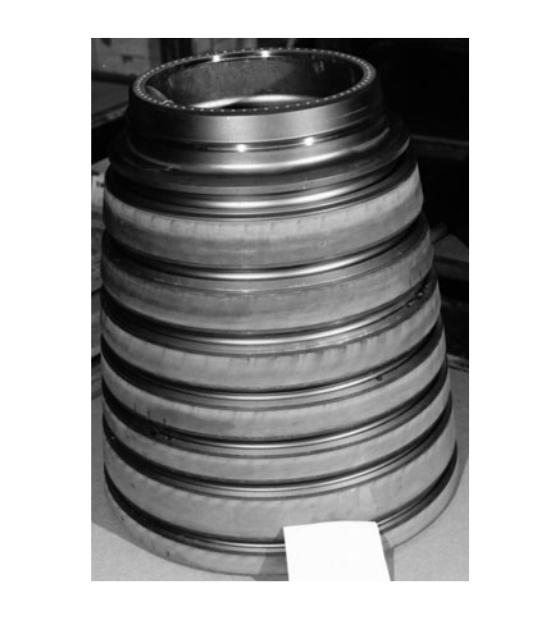
\includegraphics[width=0.9\linewidth]{./Bilder/Compressor spool}
	\caption{Verdichter für GE CF6 Triebwerk, letzte zwei Stufen Ti-6242 \cite{Prasad.2017}}
	\label{fig:compressor-spool}
\end{figure}

\begin{figure}
	\centering
	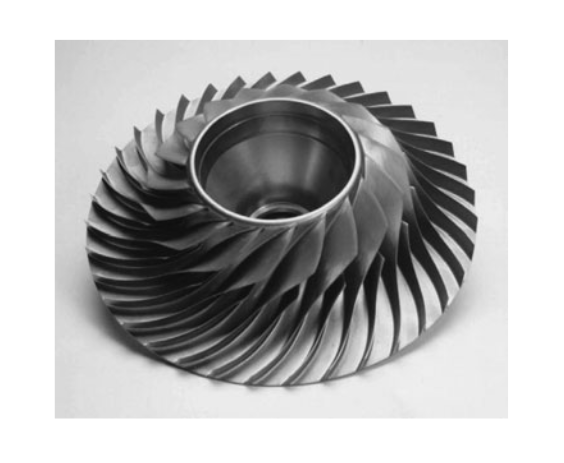
\includegraphics[width=0.7\linewidth]{./Bilder/Impeller}
	\caption{Impeller eines kleinen Triebwerks verwendet in regionalen Jets mit dem Durchmesser 35 cm, aus Ti-6242 \cite{Prasad.2017}}
	\label{fig:impeller}
\end{figure}



\begin{figure}
	\centering
	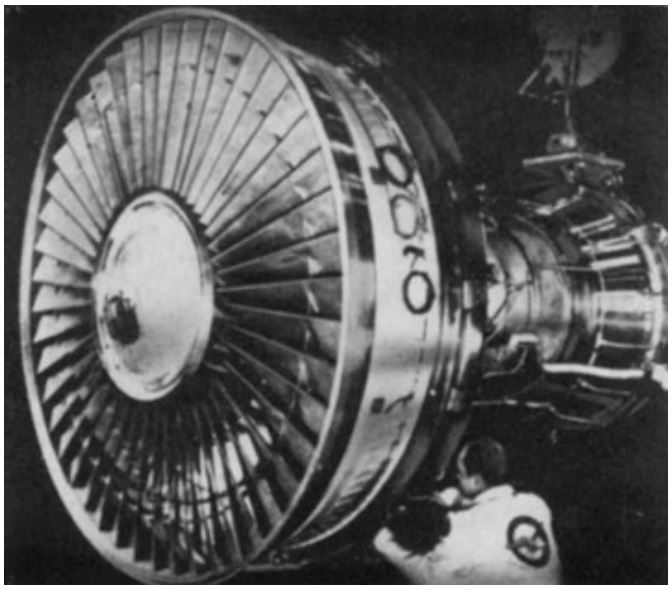
\includegraphics[width=0.6\linewidth]{Bilder/Titan}
	\caption{Bläser und Verdichter des JT9D-Triebwerkes, das zu 28 \% des Fluggewichtes aus
		Titan und Titanlegierungen besteht. Bläser aus Ti-Al6-V4. Verdichter mit zunehmender Temperatur aus TiAI6V4, Ti6242 \cite{Zwicker.2014}}
	\label{fig:titan}
\end{figure}

